\documentclass[11pt,a4paper]{article}
\usepackage[top=3cm, bottom=2cm, left=3cm, right=2cm]{geometry}
\usepackage[utf8]{inputenc}
% \usepackage[T1]{fontenc}
\usepackage{amsmath, amsfonts, amssymb}
\usepackage{siunitx}
\usepackage[brazil]{babel}
\usepackage{graphicx}
\usepackage[margin=10pt,font={small, it},labelfont=bf, textfont=it]{caption}
\usepackage[dvipsnames, svgnames]{xcolor}
\DeclareCaptionFont{MediumOrchid}{\color[svgnames]{MediumOrchid}}
\usepackage[pdftex]{hyperref}
\usepackage{natbib}
\bibliographystyle{plainnat}
\bibpunct{[}{]}{,}{s}{}{}
\usepackage{color}
\usepackage{footnote}
\usepackage{setspace}
\usepackage{booktabs}
\usepackage{multirow}
\usepackage{subfigure}
\usepackage{fancyhdr}
\usepackage{leading}
\usepackage{indentfirst}
\usepackage{wrapfig}
\usepackage{mdframed}
\usepackage{etoolbox}
\usepackage[version=4]{mhchem}
\usepackage{enumitem}
\usepackage{caption}
\usepackage{titlesec}




\titleformat{\section}{\LARGE\color{CarnationPink}}{\thesection}{1em}{}
\titleformat{\subsection}{\LARGE\color{CarnationPink}}{\thesubsection}{1em}{}


\DeclareCaptionLabelFormat{figuras}{\textcolor{CarnationPink}{Figura \arabic{figure}}}
\captionsetup[figure]{labelformat=figuras}

\makeatletter
\renewcommand\tagform@[1]{\maketag@@@{\color{CarnationPink}(#1)}}
\makeatother

\renewcommand{\theequation}{Eq. \arabic{equation}}
\renewcommand{\thefigure}{Fig. \arabic{figure}}
\renewcommand{\thesection}{\textcolor{CarnationPink}{\arabic{section}}}

\setlist[itemize]{label=\textcolor{CarnationPink}{$\mathbf{\square}$}}

\setlist[enumerate]{label=\textcolor{CarnationPink}{\arabic*.}, align=left}


\newcounter{exemplo}

\NewDocumentEnvironment{exemplo}{ O{} }{%
\allowbreak
\setlength{\parindent}{0pt}
  \begin{mdframed}[
  leftline=true,
  topline=false,
  rightline=false,
  bottomline=false,
  linewidth=2pt,
  linecolor=CarnationPink,
  frametitlerule=false,
  frametitlefont=\Large\bfseries\color{CarnationPink},
  frametitle={\color{CarnationPink}\normalfont\bfseries #1},
  ]
}{%
  \end{mdframed}
}

\setlength{\fboxsep}{5pt}
\setlength{\fboxrule}{1.5pt}
\usepackage{float}
\renewcommand{\thefootnote}{\alph{footnote}}
\usepackage{url}
\hypersetup{
	colorlinks=true,
	linkcolor=DarkTurquoise,
	filecolor=DarkTurquoise,      
	urlcolor=DarkTurquoise,
	citecolor=DarkTurquoise,
	pdftitle={Radioterapia}
}
\pagestyle{fancy}
\fancyhf{}
\renewcommand{\headrulewidth}{0pt}
\rfoot{Página \thepage}

\title{Braquiterapia}
\author{Principais Aplicadores\nocite{*}}
\date{\textit{Dalila Mendonça}}
\begin{document}
	\maketitle

    \section{Aplicadores Para Braquiterapia de Próstata}

        \subsection{Aplicador MICK}

            \begin{figure}[h]
                \centering
                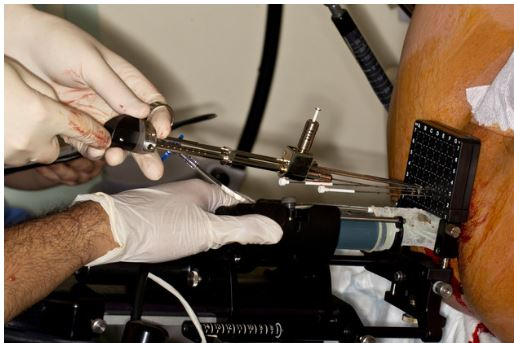
\includegraphics[width=0.5\textwidth]{Imagens/aplicadorMick.JPG}
                \caption{Aplicador Mick}
            \end{figure}

    \pagebreak
    \section{Aplicadores Para Braquiterapia Ginecológica}

        \subsection{Anel E Sonda}

            \begin{figure}[h]
                \centering
                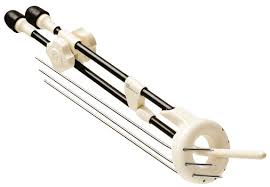
\includegraphics[width=0.5\textwidth]{Imagens/aplicadorAnelESonda.jpg}
                \caption{Anel E sonda com opções de agulhamento para serem inseridos no colo do útero}
            \end{figure}
        
        \subsection{Sonda e Ovóides}
        
            \begin{figure}[h]
                \centering
                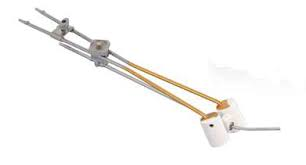
\includegraphics[width=0.5\textwidth]{Imagens/aplicadorSondaEOvoides.jpg}
                \caption{Aplicador ginecológico composto por uma sonda central e dois ovóides laterais.}
            \end{figure}

    \pagebreak
    \section{Aplicadores Para Braquiterapia De Mama}

        \subsection{Balões intramamários}

            \begin{figure}[h]
                \centering
                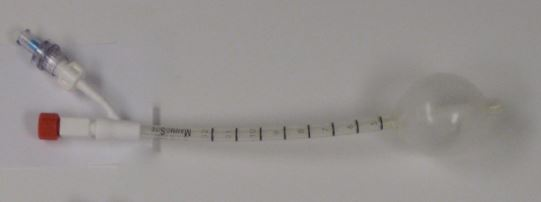
\includegraphics[width=0.5\textwidth]{Imagens/aplicadorMammoSite2.jpg}
                \caption{Aplicador MammoSite contendo um único lúmen central}
            \end{figure}

            \begin{figure}[h]
                \centering
                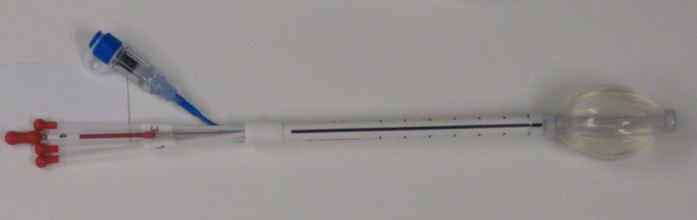
\includegraphics[width=0.5\textwidth]{Imagens/aplicadorMammositeML.JPG}
                \caption{Aplicador MammoSiteML contendo um lúmen central e 3 lúmens periféricos}
            \end{figure}

            \begin{figure}[h]
                \centering
                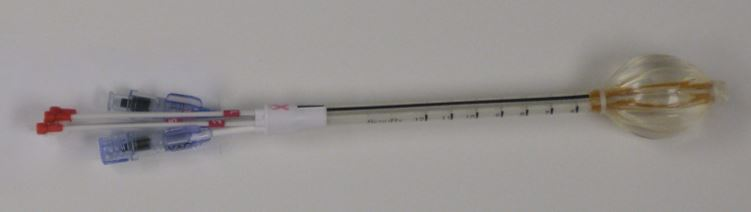
\includegraphics[width=0.5\textwidth]{Imagens/aplicadorContura2.JPG}
                \caption{Aplicador Contura contendo um lúmen central e 4 lúmens periféricos}
            \end{figure}

            \begin{figure}[h]
                \centering
                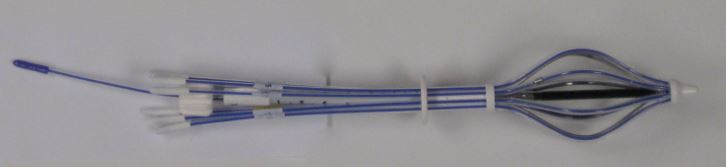
\includegraphics[width=0.5\textwidth]{Imagens/aplicadorSavi.JPG}
                \caption{Aplicador strut-based com vários lumens. Diferentemente dos demais não possui estrutura de silicone para ser inflada}
            \end{figure}


    \pagebreak
    \section{Aplicadores oftalmológicos}
            
        \subsection{Placas oftalmológicas}
            
            \begin{figure}[h]
                \centering
                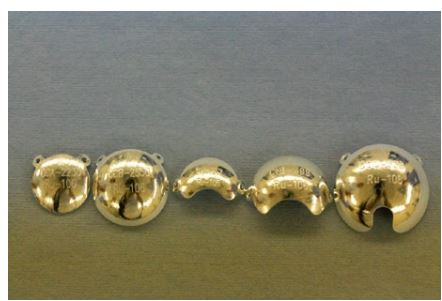
\includegraphics[width=0.5\textwidth]{Imagens/aplicadorPlacasOftamicasDeRutenio103.JPG}
                \caption{Placas oftamológicas de Rutênio 106 com diferentes tamanhos.}
            \end{figure}

            \begin{figure}[h]
                \centering
                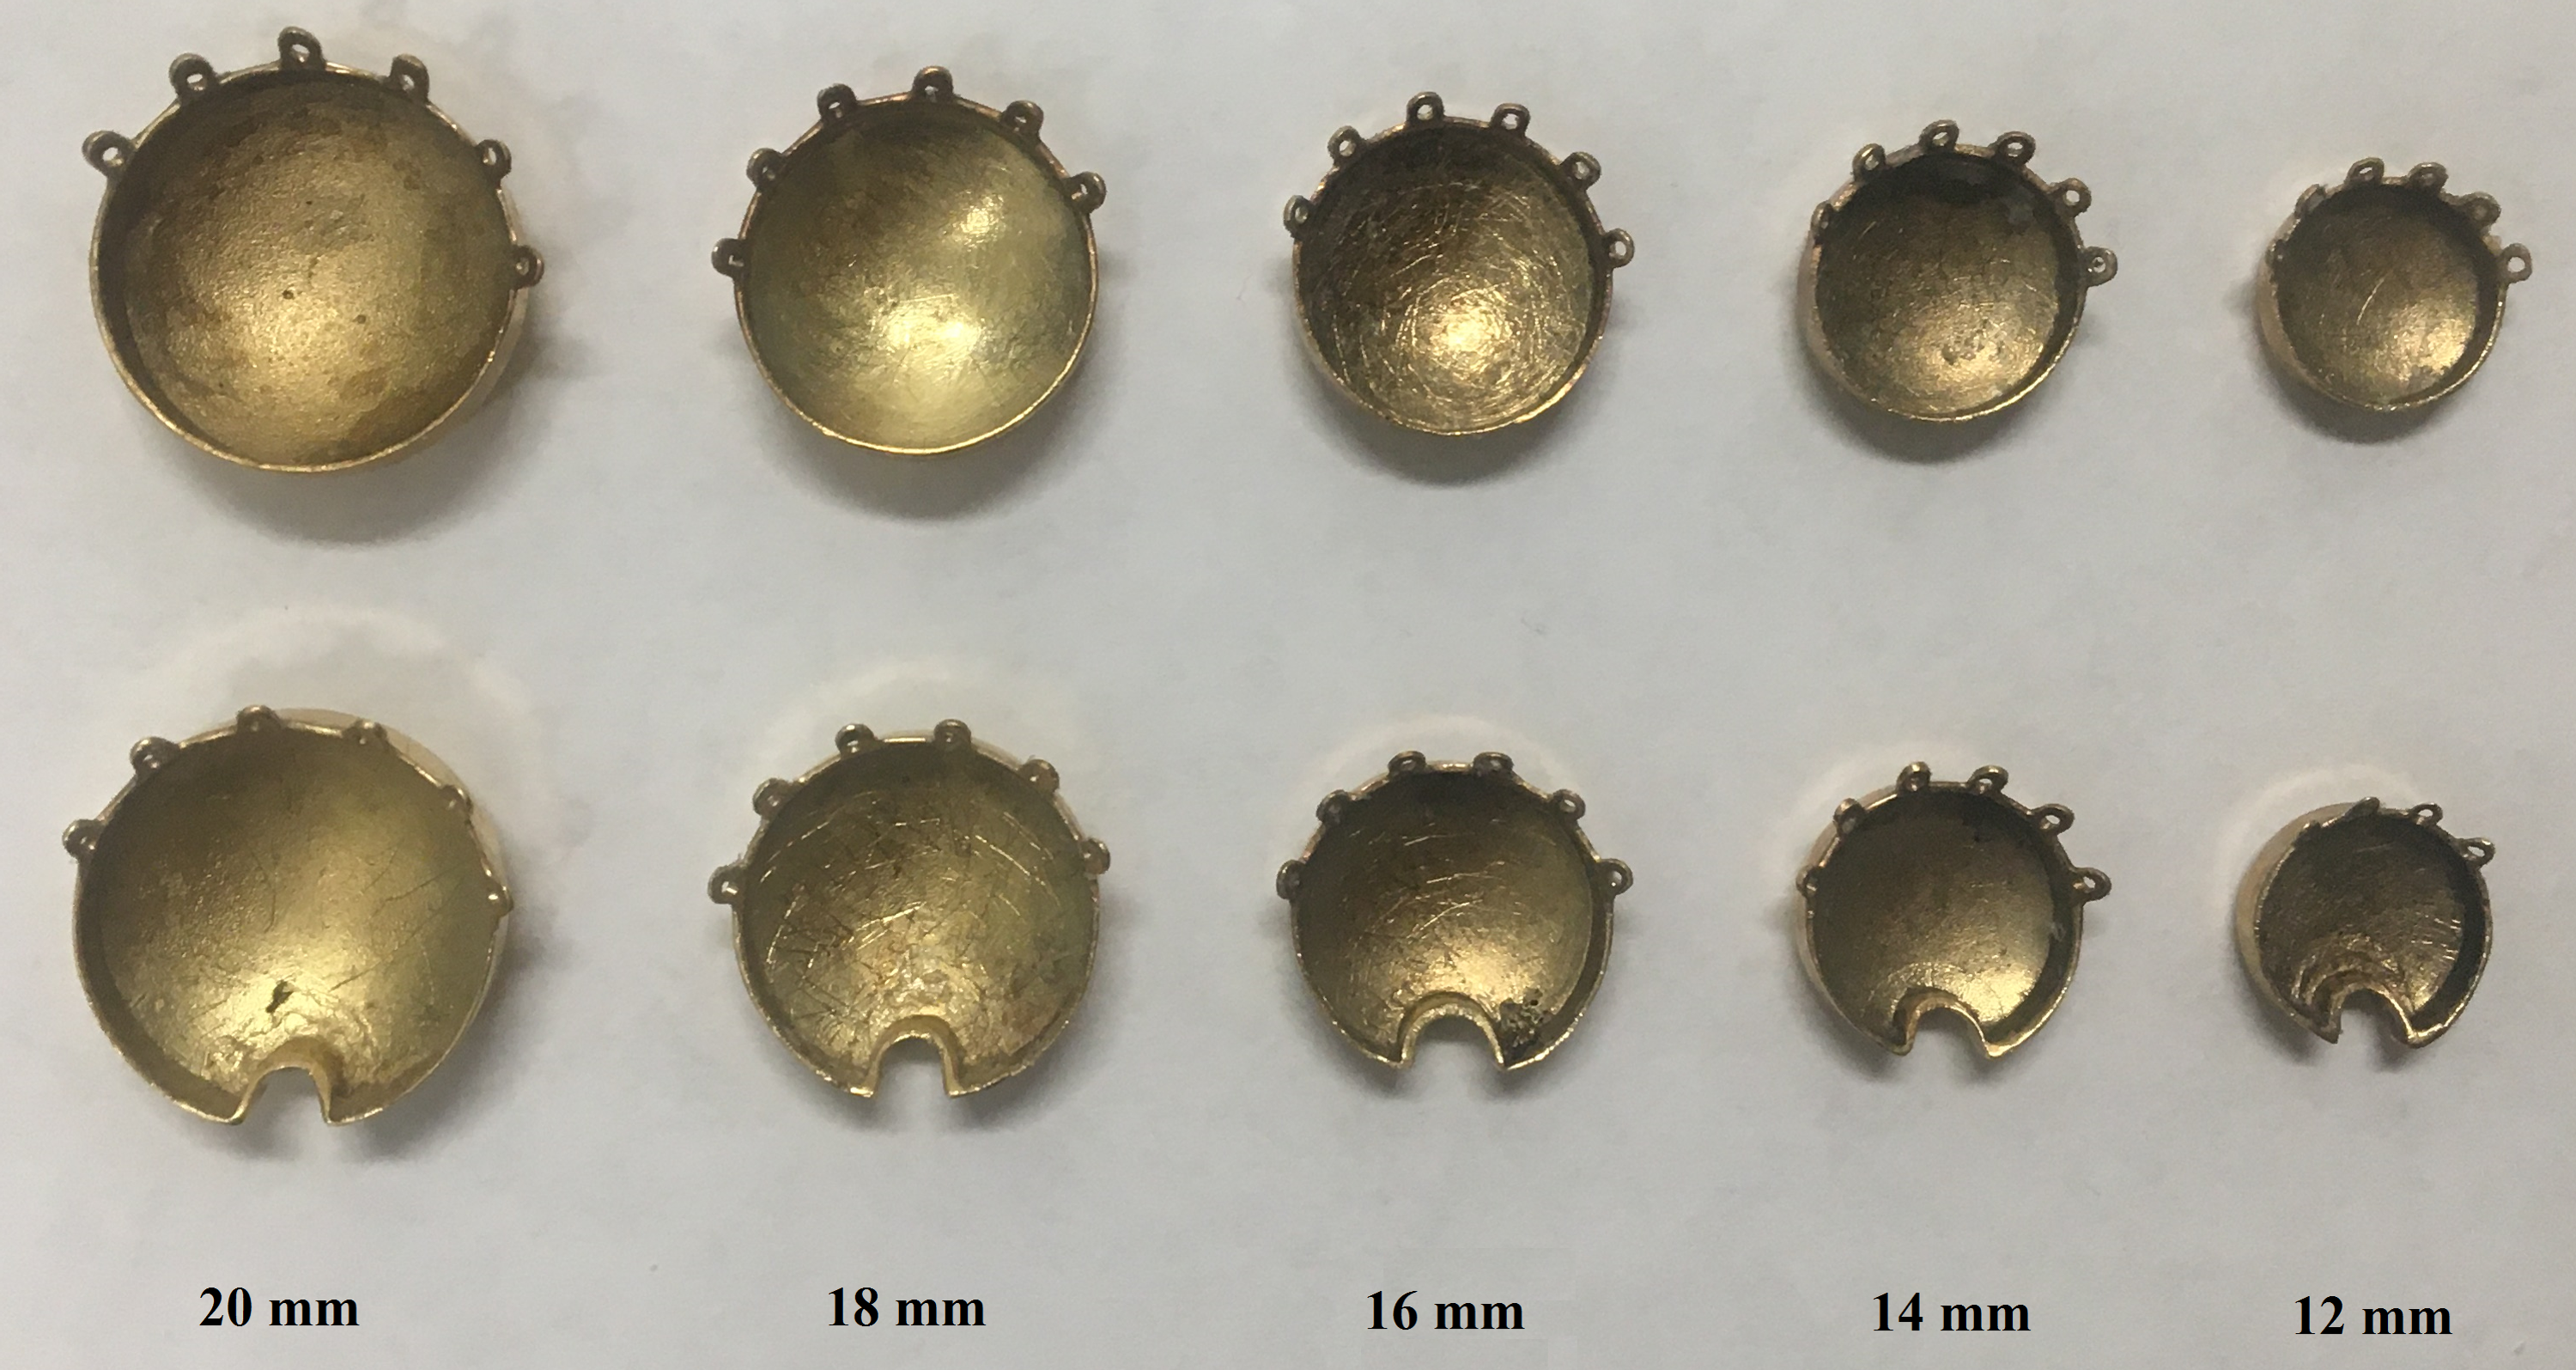
\includegraphics[width=0.5\textwidth]{Imagens/aplicadorCOMS.JPG}
                \caption{Placas oftamológicas padrão COMS confeccionadas a partir de uma capa feita de liga de ouro que recebe portatodes de fontes feitos de silicone.}
            \end{figure}

\pagebreak
\bibliography{ref.bib}  
\end{document}
